\begin{figure}[htbp]
\centering
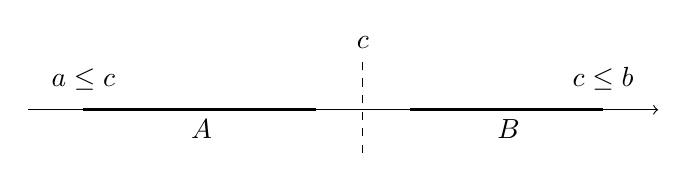
\begin{tikzpicture}[x=1cm,y=1cm]
  \draw[->] (-4,0) -- (4,0);
  \draw[very thick] (-3.3,0) -- (-0.35,0);
  \draw[very thick] (0.85,0) -- (3.3,0);
  \draw[dashed] (0.25,-0.55) -- (0.25,0.65);
  \node[below] at (-1.8,0) {$A$};
  \node[below] at (2.1,0) {$B$};
  \node[above] at (0.25,0.65) {$c$};
  \node[above] at (-3.3,0.12) {$a\le c$};
  \node[above] at (3.3,0.12) {$c\le b$};
\end{tikzpicture}
\caption{A separator $c$ lies between every point of the left set and every point of the right set.}
\end{figure}
